\documentclass[12pt,a4paper,titlepage]{report}
\usepackage{polski}
\usepackage[utf8]{inputenc}
\usepackage{amsmath}
\usepackage{amsfonts}
\usepackage{amssymb}
\usepackage{graphicx}
\usepackage{listings}
\usepackage{enumerate}
%hiperłącza
\usepackage{hyperref}
\hypersetup{
    colorlinks,
    citecolor=black,
    filecolor=black,
    linkcolor=black,
    urlcolor=black
}
%XML
\usepackage{color}
\definecolor{dkgreen}{rgb}{0,0.6,0}
\definecolor{gray}{rgb}{0.5,0.5,0.5}
\definecolor{mauve}{rgb}{0.58,0,0.82}
\definecolor{gray}{rgb}{0.4,0.4,0.4}
\definecolor{darkblue}{rgb}{0.0,0.0,0.6}
\definecolor{lightblue}{rgb}{0.0,0.0,0.9}
\definecolor{cyan}{rgb}{0.0,0.6,0.6}
\definecolor{darkred}{rgb}{0.6,0.0,0.0}


\lstset{
  	basicstyle=\ttfamily\footnotesize,
  	columns=fullflexible,
  	showstringspaces=false,
  	numbers=left,                   % where to put the line-numbers
  	numberstyle=\tiny\color{gray},  % the style that is used for the line-numbers
  	stepnumber=1,
  	numbersep=5pt,                  % how far the line-numbers are from the code
  	backgroundcolor=\color{white},      % choose the background color. You must add \usepackage{color}
  	showspaces=false,               % show spaces adding particular underscores
  	showstringspaces=false,         % underline spaces within strings
  	showtabs=false,                 % show tabs within strings adding particular underscores
  	frame=none,    
  	xleftmargin=10px,              % adds a frame around the code
  	rulecolor=\color{black},        % if not set, the frame-color may be changed on line-breaks within not-black text (e.g. commens (green 	here))
  	tabsize=2,                      % sets default tabsize to 2 spaces
  	captionpos=b,                   % sets the caption-position to bottom
  	breaklines=true,                % sets automatic line breaking
  	breakatwhitespace=false,        % sets if automatic breaks should only happen at whitespace
  	%title=\lstname,                   % show the filename of files included with \lstinputlisting;
 		                              % also try caption instead of title  
  	commentstyle=\color{gray}\upshape
}
 \lstdefinelanguage{XML}{
  	morestring=[s][\color{mauve}]{"}{"},
  	morestring=[s][\color{black}]{>}{<},
  	morecomment=[s]{<?}{?>},
  	morecomment=[s][\color{dkgreen}]{<!--}{-->},
  	stringstyle=\color{black},
  	identifierstyle=\color{lightblue},
  	keywordstyle=\color{red},
  	morekeywords={xmlns,xsi,noNamespaceSchemaLocation,type,id,x,y,source,target,version,tool,transRef,roleRef,objective,eventually},
}


\author{Katarzyna Węgiełek \\ Paweł Własiuk \\ Kamil Sienkiewicz\\ Marcin Wardziński}
\title{\textbf{Computational Cluster}}
\linespread{1.125}

\begin{document}
	\maketitle
	\tableofcontents
	
	\chapter{Wstęp}
	Tematem projektu jest stworzenie dokumentacji dla klastra obliczeniowego. Zadaniem projektowanego przez nas systemu będzie prowadzenie obliczeń rozproszonych. Klaster będzie umożliwiał rozwiązywanie skomplikowanych problemów, wykorzystujących algorytmy o dużej złożoności czasowej, w szczególności rzędu o($2^n$). Jego najważniejszą rolą będzie odpowiednie rozdzielenie zadań pomiędzy różne elementy systemu tak, aby jak najbardziej optymalnie wykorzystywać moc obliczeniową komputerów, z których się składa. Istotne jest również zminimalizowanie ryzyka utraty danych w przypadku awarii któregoś z komponentów.
	
	\section{Elementy klastra obliczeniowego}
	\textbf{Task manager} - dzieli zadanie na podproblemy i oblicza rozwiązanie końcowe na podstawie rozwiązań częściowych\\\\
\textbf{Computational node} - rozwiązuje pojedynczy podproblem i odsyła do jego rozwiązanie częściowe do communications server'a\\\\
\textbf{Communications server} - przesyła podproblemy i rozwiązania częściowe między task manager'ami a computational node'ami oraz wysyła rozwiązanie zadania do computational client'a\\\\
\textbf{Computational client} - wysyła problem do communications server'a i oczekuje na otrzymanie rozwiązania\\\\
\textbf{Task solver} - moduł używany przez computational node do rozwiązania podproblemu oraz przez task manager do podzielenia zadania i znalezienia ostatecznego rozwiązania na podstawie wyników częściowych\\
	
	\chapter{Opis działania systemu}
	Proces rozwiązywania zadania rozpoczyna się od wprowadzenia przez użytkownika danych wejściowych dla problemu. Robi to za pośrednictwem \emph{computational client'a}. Jest to jedyny element klastra, z którym użytkownik ma bezpośredni kontakt. \emph{Computational client} przetwarza wprowadzone informacje na komunikat i wysyła do \emph{communications server'a} w formie pliku XML. Następnie zadanie trafia do kolejki zgłoszonych problemów. Jeśli istnieje w danej chwili w klastrze wolny \emph{task manager}, który potrafi obsłużyć zadanie tego typu, to \emph{communications server} wysyła do niego otrzymane dane wejściowe. \emph{Task manager} dzieli problem na mniejsze części - podproblemy, przeznaczone do rozwiązania przez pojedyncze \emph{computational node'y} i odsyła je do \emph{server'a}. To czy \emph{task manager} może podzielić dany problem zależy od tego, czy posiada \emph{task solver}, zajmujący się poszukiwaną klasą problemów. \emph{Communications server} wysyła odebrane podproblemy kolejno do wolnych \emph{computational node'ów}, które są w stanie je rozwiązać (zawierają odpowiedni \emph{task solver}). \emph{Node'y} prowadzą obliczenia równolegle, a następnie wysyłają uzyskane wyniki do \emph{server'a}. \emph{Communications server} przesyła rozwiązania częściowe do \emph{task managera}, który oblicza na ich podstawie ostateczny wynik. \emph{Task manager} nie czeka aż wszystkie \emph{node'y} zakończą obliczenia - zaczyna scalanie już po otrzymaniu pierwszych rozwiązań częściowych i aktualizuje rozwiązanie za każdym razem, gdy otrzyma kolejne dane z \emph{server'a}. W niektórych typach zadań może się zdarzyć, że wyniki uzyskane przez \emph{task manager'a} po scaleniu części rozwiązań spowodują zmiany w podziale na podproblemy - np. części z nich nie będzie się już opłacało rozwiązywać, bo wiadomo będzie, że nie wpłyną na ostateczny wynik. Gdy \emph{task manager} uzyska końcowe rozwiązanie, wysyła je do \emph{server'a}. Trafia ono do kolejki zadań oczekujących na odebranie wyników. Kiedy \emph{computational client} wyśle do \emph{server'a} żądanie pobrania rozwiązania, \emph{server} odsyła mu odpowiednie dane.\\
Podczas całego procesu główny \emph{communications server} synchronizuje trzymane przez siebie dane z \emph{server'em backup'owym}, aby w razie awarii nie stracić części rozwiązań i zgłoszonych zadań. Jeśli \emph{server} główny ulegnie uszkodzeniu i komunikacja z nim będzie niemożliwa, pozostałe komponenty nie przerwą swojej normalnej pracy i zaczną wymieniać komunikaty z \emph{server'em backup'owym}.

	\section{Diagram aktywności dla rozwiązania pojedynczego problemu}
	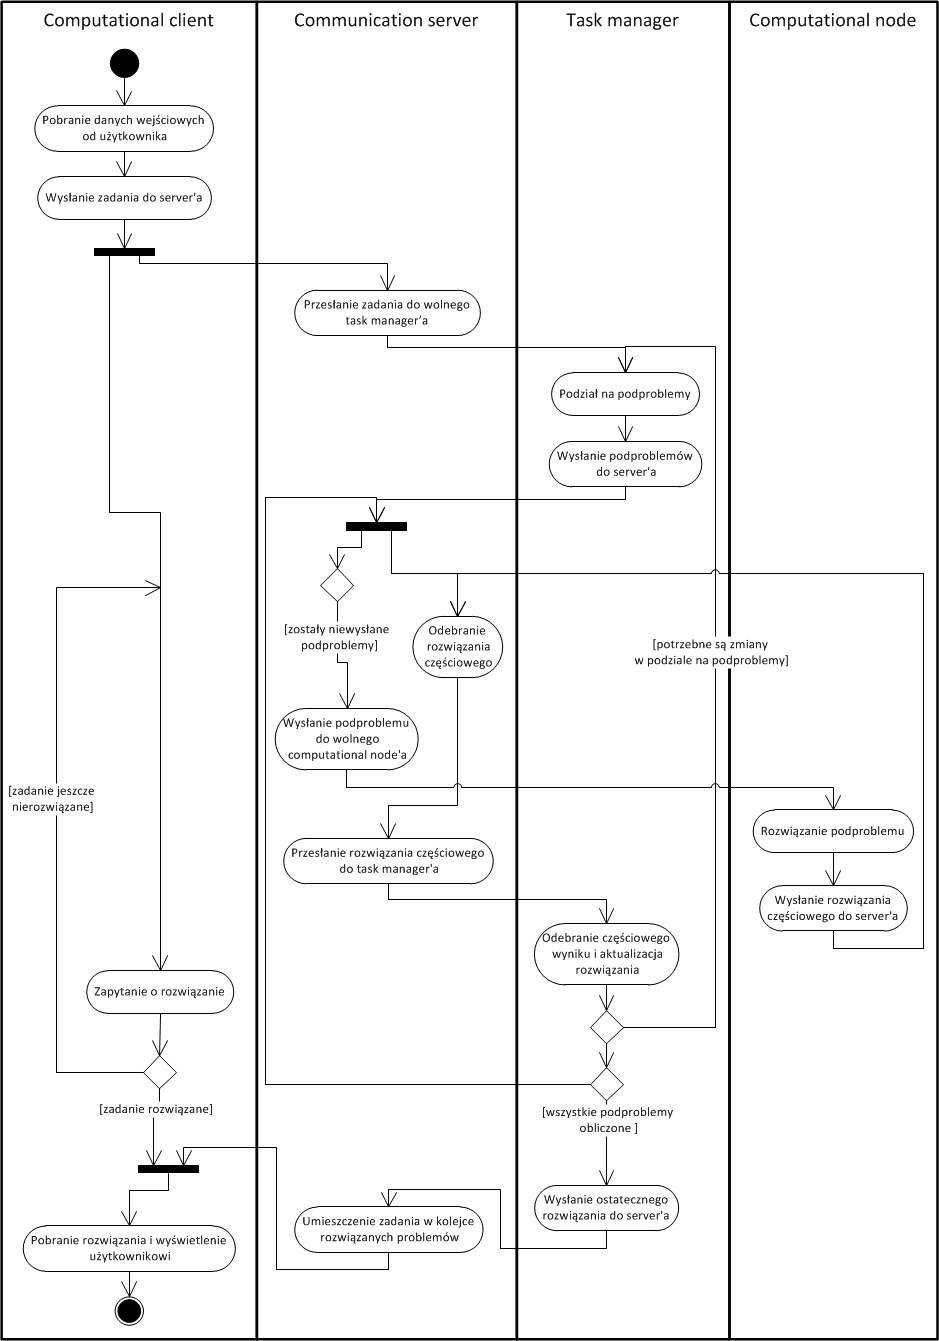
\includegraphics[width=\textwidth]{img/activityDiagram.png}
	
	\section{Diagramy przypadków użycia}	
	
	%komunikacja + schemy
	\chapter{Komunikacja}
		\section{Nawiązywania połączenia}
	Uruchomienie całego systemu rozpoczyna się od uruchomienia \textit{serwera komunikacyjnego}. Od tej chwili komponenty systemu tj. 
	\textit{węzły obliczeniowe}	i \textit{menadżery zadań} mogą zgłaszać swoją obecność w klastrze. Każdy z komponentów systemu 
	posiada w swoim pliku konfiguracyjnym (w węzłach \verb+MainServerAddress+ i \verb+BackupServerAddress+) \textbf{adres IP} i
	 \textbf{port} \textit{serwera komunikacyjnego} oraz serwera zapasowego. Zaraz po uruchomieniu każdy komponent
	zgłasza swoją obecność do głównego \textit{serwera komunikacyjnego}. Po trzech nieudanych próbach nawiązania połączenia następuje
	wysłanie identycznej informacji do serwera backup'owego. Każdy z komponentów w takiej wiadomości informuje o swoim rodzaju podaje
	IP i port na którym	działa. Na tej podstawie serwer będzie komunikował się z tymi elementami systemu.\\
	
		 \lstinputlisting[caption=\footnotesize{Wiadomość wysyłana przez komponent włączający się do systemu},language=XML,firstline=1,lastline=6]{examples.xml} 
		
	Parametr \verb+ComponentType+ informuje o rodzaju komponentu systemu. Wartości, które może przyjąć ten parametr to:
	\begin{itemize}
		\item \verb+TaskManager+ - w przypadku gdy wiadomość pochodzi od \textit{menadżera zadań},
		\item \verb+ComputationalNode+ - gdy wiadomość pochodzi od \textit{węzła obliczeniowego}
	\end{itemize} 

	Zadaniem \textit{serwera komunikacyjnego} jest utrzymywanie listy aktywnych komponentów systemu, oraz przechowywanie informacji
	na temat klas problemów, które dane komponenty obsługują. W tym celu serwer regularnie, co pewien określony czas
	będzie odpytywał wszystkie swoje komponenty prosząc o listę klas problemów możliwych do rozwiązania. W przypadku gdy takiej
	odpowiedzi nie otrzyma uznaje komponent za wyłączony i usuwa jego dane z pamięci. W przypadku otrzymania odpowiedzi na
	żądanie, \textit{serwer} na podstawie otrzymanych danych uzupełnia/aktualizuje informacje o rozwiązywalnych problemach
	przez komponenty.\\
	
		\lstinputlisting[caption=\footnotesize{Odpowiedź komponentu na żądanie serwera},language=XML,firstline=8,lastline=14]{examples.xml} 

	W wiadomości, dla każdego typu problemu zostają przekazane dwie informacje:
	\begin{itemize}
		\item \verb+problemClassName+ - nazwa problemu,
		\item \verb+problemClassId+ - guid problemu, który w jednoznaczny sposób identyfikuje typ problemu.	
	\end{itemize} 		
		
	\begin{figure}[h]
		\centering
		\caption{Uzyskiwanie połączenia przez komponent systemu}
		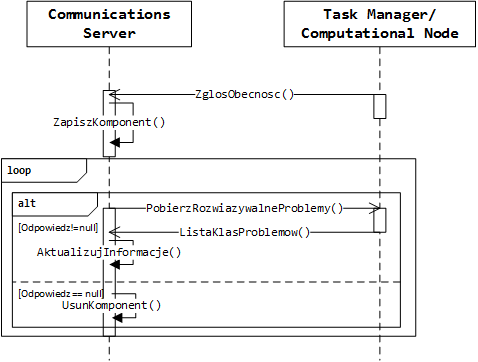
\includegraphics[width=0.8\textwidth]{img/communication/connecting.png}
	\end{figure}
	
	\section{Lista rozwiązywalnych problemów}
	Proces rozwiązywania zadania przez \textit{klaster obliczeniowy} rozpoczyna się na poziomie aplikacji klienckiej. Przed
	wysłaniem problemu do rozwiązania, aplikacja kliencka musi pobrać z serwera informację na temat klas problemów
	rozwiązywalnych w danej chwili przez klaster obliczeniowy (wynika ona z obecnie dostępnych \textit{Menadżerów zadań} i
	\textit{węzłów obliczeniowych}). Aplikacja kliencka odpytuje \textit{serwer komunikacyjny} o potrzebne informacje. 
	\textit{Serwer} w odpowiedzi na to żądanie odsyła wiadomość, w której zawarte są informacje o wszystkich typach problemów
	rozwiązywalnych przez klaster. Informacje zostają przetworzone i przedstawione użytkownikowi. Wiadomość przesłana do 
	\textit{aplikacji klienckiej} jest identyczna z tą, którą serwer otrzymuje od pozostałych komponentów systemu.
	
	\begin{figure}[h]
		\centering
		\caption{Diagram sekwencji pobierania informacji z serwera przez aplikację kliencką}
		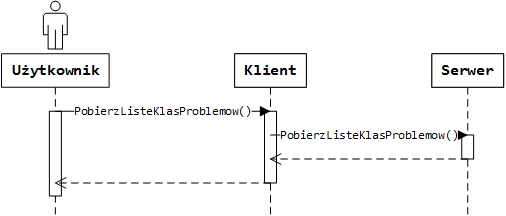
\includegraphics[width=0.9\textwidth]{img/communication/problemclass.png}
	\end{figure}	
	
	\section{Rozwiązywanie zadania}
	
	Po wykonaniu czynności opisanych w poprzednim rozdziale, użytkownik może zlecić zadanie \textit{klastrowi obliczeniowemu}
    \textit{Aplikacja kliencka} wysyła do serwera wiadomość z informacją o typie rozwiązywanego problemu i dane wejściowe zadania.\\
    
    \lstinputlisting[caption=\footnotesize{Zlecenie rozwiązania zadania przez aplikację kliencką},language=XML,firstline=16,lastline=20]{examples.xml}
    
     Wiadomość zawiera 2 parametry konieczne do stworzenia i rozwiązania zadania:
    \begin{itemize}
    	\item \verb+problemClassId+ - identyfikator klasy problemu, umożliwiający zidentyfikowanie, które części systemu są w stanie rozwiązać dany problem
    	\item \verb+Data+ - parametry typu \verb+String+ zawierający dane wejściowe dla danego typu problemu. Dane te przedstawione 
    					są w formacie XML odpowiednim dla danego typu problemu.  
    \end{itemize}
    
    Serwer po otrzymaniu wiadomości generuje specjalny identyfikator, który przypisuje do zadania. Będzie on wykorzystany do 
    identyfikacji poszczególnych podzadań oraz umożliwi klientowi zidentyfikowanie zleconego zadania.\\
    
    \lstinputlisting[caption=\footnotesize{Informacja z tokenem zwracana do aplikacji klienckiej},language=XML,firstline=22,lastline=25]{examples.xml}
    
    Taki token zostaje również odesłany do aplikacji klienckiej, która zapisze go w swoim pliku konfiguracyjnym. Poniżej przykład prezentujący odpowiedni wpis:
    
    \begin{lstlisting}[language=XML,numbers=none]
    <TaskList>
    	<Task taskname="customTaskName1" taskToken="ee28fec2-6361-4a58-aaf1-b9ff0f509743"/>
    	<Task taskname="customTaskName2" taskToken="4fbcbba1-014e-4643-b60f-f7888a95bb54"/>
    </TaskList>
    \end{lstlisting}
    Węzeł \verb+Task+ odpowiada jednemu zleconemu zadaniu przez użytkownika. Każdy taki węzeł posiada dwa atrybuty:
	
	\begin{itemize}
		\item \verb+taskToken+ - to identyfikator zadania nadany przez klaster obliczeniowy, dzięki niemu użytkownik będzie miał możliwość pobrania rozwiązania zadania,
		\item \verb+taskname+ - nazwa zadania nadana przez użytkownika, która umożliwi mu zidentyfikowanie zadania, nazwa obecna wyłącznie na poziomie aplikacji klienckiej.
	\end{itemize}	    
      
	
	\begin{figure}[h]
		\centering
		\caption{Diagram sekwencji pobierania informacji z serwera przez aplikację kliencką}
		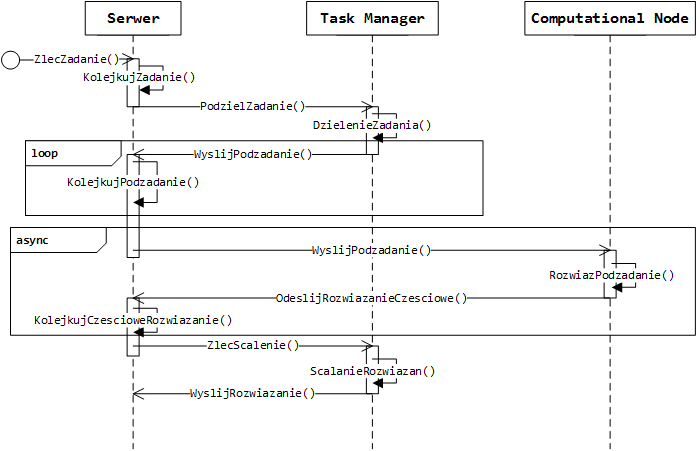
\includegraphics[width=\textwidth]{img/communication/computation.png}
	\end{figure}    
    
    
    Klaster obliczeniowy wykonuje ciąg czynności koniecznych do otrzymania rozwiązania, tzn:
	\begin{enumerate}[(1)]
		\item przesłanie polecenia podziału zadania od \textit{serwera} do \textit{menadżera zadań} - wiadomość w formacie otrzymanym od
		\textit{aplikacji klienckiej},
		\item podział zadania i odesłanie stworzonych podproblemów prowadzących do otrzymania rozwiązania. \textit{Menadżer zadań} dokonuje podziału zadania, każdemu z nich przydzielając unikalny identyfikator. Wiadomość zwrotna zawiera informacje o 
		typie rozwiązywalnego problemu, identyfikatora zadania, identyfikatora podzadania, oraz danych wejściowych potrzebnych do rozwiązania zadania.
		
		\lstinputlisting[caption=\footnotesize{Zlecenie podzadania},language=XML,firstline=36,lastline=42]{examples.xml}
		
		\item przesłanie każdego z podzadań do \textit{węzłów obliczeniowych}
		\item przeprowadzenie obliczeń i odesłanie częściowych rozwiązań do \textit{serwera}. Odsyłana wiadomość zawiera informacje o 
		typie rozwiązywalnego podproblemu, identyfikatorze zadania, identyfikatorze podzadania oraz rozwiązaniu częściowym problemu.
		\item przesłanie częsciowych rozwiązań do \textit{menadżera zadań} w celu stworzenia rozwiązania. Przesłanie waidomości wcześniej zebranych od \textit{węzłów obliczeniowych}.
		\item odesłanie pełnego rozwiązania zadania do \textit{serwera} w identycznym formacie jak te, które serwer odsyła do \textit{aplikacji klienckiej}
	\end{enumerate}

	Zadanie przesłane do podziału przez \textit{serwer komunikacyjny} jest w formacie otrzymanym od \textit{aplikacji klienckiej}    
    
    \section{Odczytanie rozwiązania}	
	Proces odczytywania rozwiązania zadania rozpoczyna się od załadowania listy zadań zleconych przez daną aplikację z pliku konfiguracyjnego do którego wcześniej zostały wpisane identyfikatory poszczególnych zadań. Użytkownik wybiera zadanie którego rozwiązanie
	chce pobrać. Aplikacja odpytuje serwer o rozwiązanie, w wyniku czego otrzymuje informację na jego temat. Wiadomość, którą wysyła aplikacja kliencka w węźle \verb+TaskId+ zawiera identyfikator zadania którego rozwiązania oczekujemy.\\

	 \lstinputlisting[caption=\footnotesize{Rozwiązanie zadania},language=XML,firstline=28,lastline=34]{examples.xml}

	\begin{figure}[h]
		\centering
		\caption{Diagram sekwencji pobierania informacji z serwera przez aplikację kliencką}
		 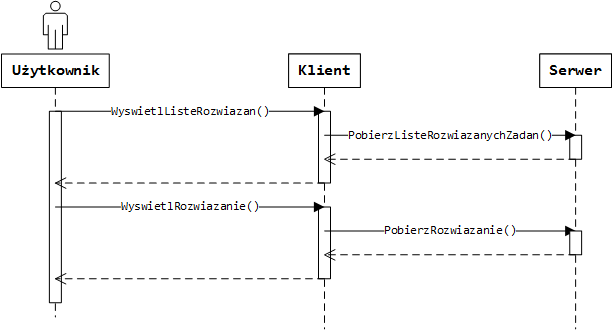
\includegraphics[width=\textwidth]{img/communication/getresult.png}
	\end{figure} 	
	
	Wiadomość otrzymana od serwera składa się z 4 węzłów:
	\begin{itemize}
		\item \verb+problemClassId+ - identyfikator klasy problemów, której dotyczy zadanie. Informacja potrzebna do odpowiedniego wyboru 
		pluginu, który odpowiednio sparsuje i przedstawi wyniki użytkownikowi.
		\item \verb+TaskId+ - identyfikator zadania
		\item \verb+Status+ - dwie możliwe wartości to \verb+Done+ - jeżeli zadanie zostało ukończone oraz \verb+InProgress+ - jeżeli rozwiązywanie zadania nadal trwa.
		\item \verb+Data+ - w przypadku gdy status przyjmuję wartość \verb+Done+ pole zawiera rozwiązanie zadania w postaci XML,
		w przeciwnym przypadku wartość jest pusta
	\end{itemize}
	
	
	\section{Schema}
		\subsection{Uzyskiwanie połączenia przez komponenty}	
			\lstinputlisting[language=XML]{schema/connectionMessageSchema.xsd}
		\subsection{Lista rozwiązywalnych problemów przez klaster obliczeniowy}
			\lstinputlisting[language=XML]{schema/SolvableProblemListMessage.xsd}
		\subsection{Zlecenie rozwiązania zadania}
			\lstinputlisting[language=XML]{schema/TaskOrderMessage.xsd}
		\subsection{Token wysyłany do aplikacji klienckiej}
			\lstinputlisting[language=XML]{schema/TaskTokenMessage.xsd}
		\subsection{Żądanie o przesłanie rozwiązania zadania}
			\lstinputlisting[language=XML]{schema/TaskResultRequestMessage.xsd}
		\subsection{Rozwiązanie Zadania}
			\lstinputlisting[language=XML]{schema/TaskResultMessage.xsd}
		\subsection{Zlecenie rozwiązania podzadania}
			\lstinputlisting[language=XML]{schema/SubtaskOrderMessage.xsd}
		\subsection{Przesłanie rozwiązania podzadania}
			\lstinputlisting[language=XML]{schema/SubtaskResultMessage.xsd}
\end{document}